% \documentclass{article}


% Options for packages loaded elsewhere
%\PassOptionsToPackage{unicode}{hyperref}

\documentclass[
]{article}
%\usepackage{amsmath,amssymb}
\author{}
\date{}

\usepackage{geometry}
\geometry{
    a4paper,
    left=30mm,
    right=30mm,
    top=30mm,
    bottom=30mm,
}

\usepackage[footnotes,definitionLists,hashEnumerators,smartEllipses,hybrid]{markdown}
\usepackage[utf8]{inputenc}
\usepackage[document]{ragged2e} % remove line justify
\usepackage{dblfloatfix}
\usepackage{microtype}
\usepackage[none]{hyphenat}
\usepackage{setspace}
\setstretch{1.2} % Optionally adjust line spacing

\setlength{\RaggedRightParindent}{\parindent}
\setlength{\parskip}{1em}
  
\usepackage{fontspec}
%\defaultfontfeatures{Mapping=tex-text,Scale=MatchLowercase}
\setmainfont{Source Sans Pro--Light}[BoldFont={Source Sans Pro-Regular}, ItalicFont={Source Sans Pro-Light Italic},]

\usepackage{xurl} % for '\url' macro
\usepackage{xcolor}
\definecolor{kispiblack}{HTML}{333333}
\definecolor{kispidarkblue}{HTML}{023047}
\definecolor{kispidarkgreen}{HTML}{006666}
\definecolor{kispired}{HTML}{C70000}
\definecolor{kispilink}{HTML}{007DB8}%219EBC
% \color{kispi_black} %default

% command to use these colors and formatting; xspace for correct spacing including with punctuation marks.
\usepackage{xspace}
\newcommand{\variablesdarkgreen}[1]{\textbf{\textcolor{kispidarkgreen}{#1}}\xspace}

% \color{kispiblack} 

 % green #219EBC
% darkgreen #006666

\usepackage{authblk}
\usepackage{lineno}
\usepackage{enumitem}
\setlist[itemize]{noitemsep}

\usepackage{siunitx} % SI units


\usepackage[colorlinks]{hyperref}
\hypersetup{
    linkcolor={kispilink},
    citecolor={kispilink},
    filecolor=blue!50!black,
    urlcolor=kispilink,
}

\usepackage{natbib}
\setcitestyle{square,numbers,sort&compress}
\usepackage{hypernat}

\usepackage{graphicx}
\graphicspath{ {images/} }

\usepackage{booktabs}
\usepackage{rotating, tabularx}
\usepackage{ltablex}
\usepackage{caption}
\captionsetup{font=normalsize}

\usepackage{pdflscape}
\usepackage{multirow}

\usepackage{fancyhdr}
\pagestyle{fancy}
%\lhead{Lecture 1}
%\rhead{Handout 1}
%\lfoot{Lecture 1}
%\rfoot{Handout 1}
\usepackage{tocloft}  % Customizing the Table of Contents
\setcounter{tocdepth}{1}

% cover

%\usepackage[a4paper,margin=5pt]{geometry}



\newcommand{\SampleID}{XYZ\_STUDY\_D.XYZ003\_DNA}
\newcommand{\CodingVariant}{ENST00000380588.4:c.53G>A}
\newcommand{\ProteinVariant}{ENSP00000369962.4:p.Trp18Ter}


% Precision Medicine Unit
\newcommand{\pmu}{\variablesdarkgreen{Precision medicine unit}}
\newcommand{\kispi}{\variablesdarkgreen{Universitäts-Kinderspital Zürich}}

% Products
\newcommand{\acmguru}{\variablesdarkgreen{ACMGuru (v1.0)}}
\newcommand{\deepinfer}{\variablesdarkgreen{DeepInfeR (v1.0)}}
\newcommand{\archipelago}{\variablesdarkgreen{Archipelago (v1.0)}}
\newcommand{\skatrbrain}{\variablesdarkgreen{SkatRbrain (v0.2)}}
\newcommand{\macat}{\variablesdarkgreen{multi-omic ACAT (v0.1)}}
\newcommand{\dnasnake}{\variablesdarkgreen{DNAsnake (v0.1)}}
\newcommand{\rnasnake}{\variablesdarkgreen{RNAsnake (v0.1)}}

% Documentation
\newcommand{\pipedevdocdna}{\variablesdarkgreen{Pipe-Dev docs \dnasnake}}


% IVDR Compliance Documentation Variables

% Reference Genome
\newcommand{\referenceGenome}{\variablesdarkgreen{GRCh38.p13}}
\newcommand{\referenceGenomeVersion}{\variablesdarkgreen{GCA\_000001405.15\_GRCh38\_no\_alt\_analysis\_set}}
\newcommand{\referenceGenomeSource}{\variablesdarkgreen{\url{ftp://ftp.ncbi.nlm.nih.gov/genomes/all/GCA/000/001/405/GCA_000001405.15_GRCh38/seqs_for_alignment_pipelines.ucsc_ids/GCA_000001405.15_GRCh38_no_alt_analysis_set.fna.gz}}}
\newcommand{\referenceGenomeDoc}{\variablesdarkgreen{https://swisspedhealth-pipelinedev.github.io/docs/pages/ref.html}}

% Git Repositories
\newcommand{\gitRepoDNAsnake}{\variablesdarkgreen{\url{https://github.com/SwissPedHealth-PipelineDev/docs}}}
\newcommand{\gitRepoDNAsnakeCommit}{\variablesdarkgreen{581d0ed0f67ad86669ffcb2d2a03f22638fda1ae}}
\newcommand{\gitRepoDNAsnakeTag}{\variablesdarkgreen{v0.1}}

\newcommand{\gitRepoGATK}{\variablesdarkgreen{\url{https://github.com/broadinstitute/gatk}}}
\newcommand{\gitRepoGATKCommit}{\variablesdarkgreen{59c9c1bba1c3edf6624468fd4f81f4fa2fe3fbae}}

\newcommand{\gitRepoVEP}{\variablesdarkgreen{\url{https://github.com/Ensembl/VEP_plugins}}}
\newcommand{\gitRepoVEPCommit}{\variablesdarkgreen{74c9315623660e622effb7572c1ed21e6700c2ea}}

% Compliance Tags
\newcommand{\ivdrCompliantTag}{\variablesdarkgreen{IVDR\_Compliant}}
\newcommand{\qualityControlPassed}{\variablesdarkgreen{QC\_Passed}}

% Metadata and Document Control
\newcommand{\documentID}{\variablesdarkgreen{DS-IVDR-003}}
\newcommand{\documentVersion}{\variablesdarkgreen{1.2}}



\newcommand{\documentversion}{Labhart-Schwyzer}
\lhead{GenomeSwift}
\rhead{}
% \lfoot{\date{\today}}
\rfoot{\documentversion}
\usepackage{titlesec}
% Adjust spacing for \section
\titlespacing*{\section}
{0pt} % indent from the left margin
{0pt plus 0pt minus 6pt}
{0pt plus 0pt minus 6pt} 

% Adjust spacing for \subsection
\titlespacing*{\subsection}
{0pt} % indent from the left margin
{0pt plus 0pt minus 6pt}
{0pt plus 0pt minus 6pt} 

% Adjust spacing for \subsubsection
\titlespacing*{\subsubsection}
{0pt} % indent from the left margin
{0pt plus 0pt minus 6pt}
{0pt plus 0pt minus 6pt} 

\usepackage{float} % Include this in the preamble if not already included



\begin{document}


%x Project Title (0.25 page)
%x Summary (0.25 page)
%x Introduction and Background (≈ 1 page)
%x Objectives of the Project (≈ 0.5 pages)
%Methods and Materials (≈ 0.5 page)
%Expected Outcomes and Significance (≈ 0.25 pages)
%Added Value for the Applicant's Career and Home Institution (≈ 0.5 pages)
%x Collaborations and Network (≈ 0.25 pages)
%Ethics and Data Protection (0.25 page)
%x Timeline and Milestones (≈ 0.25 pages)
%x Financial Plan and Budget (≈ 0.5 pages)
%x References (0.25 page)
%
%
%5 Scholarship benefits
%The funding amount is CHF 66,000 and is thus based on the rates of the Swiss National Science Foundation for postdoctoral mobility fellowships. 
% 
%6 Use of the funding
%The funding is intended to cover travel costs, accommodation and research expenses incurred during the research stay.

\tableofcontents  % This line adds the table of contents

\newpage  % Starts a new page after the table of contents

\begin{figure}[H] % Ensures that the figure is placed exactly where it appears in the code
  \begin{flushright} % Aligns the image to the right
    \vspace{-1em} % Adjusts the vertical position, lifting the image up
    
\includegraphics[width=0.1\textwidth]{../../resources/images/genome_swift/genome_swift_logo.png}
    \vspace{-4em} % Reduces the vertical space below the image to allow text to flow beneath it
  \end{flushright}
\end{figure}

\section*{GenomeSwift}
\textbf{Precision medicine in through rapid and automated multi-omic analysis}.

\section{Summary}

\textbf{Background}: The integration of advanced genomic technologies into healthcare, particularly for rare genetic diseases, is crucial for improving diagnostic and treatment strategies. The current fragmented analysis methodologies delay critical medical responses. Our proposal aims to streamline and automate these processes. This can provide a new opportunity for precision medicine in Kispi by offering rapid, precise insights into genetic disorders.

\textbf{Objective}: The primary goal of GenomeSwift is to develop and deploy a comprehensive, automated software pipeline that enhances the speed and accuracy of genomic data analysis, particularly for diagnosing and treating genetic diseases in Kispi.

\textbf{Research Plan}: GenomeSwift will integrate several purpose-build tools (ProteoMCLustR, SkatRbrain, Archipelago, ACMGuru, and DeepInferR), along with several industry-standards, into one unified platform to optimise genomic data processing from initial input to clinical interpretation. The project will employ robust statistical methodologies and simulation/validation processes to ensure reliability and clinical relevance.

\textbf{Relevance/Significance}: By enhancing genomic analysis capabilities, GenomeSwift aligns with Kispi’s strategic goals and addresses an unmet need in personalised medicine. It promises to reduce the time to diagnosis and treatment, significantly impacting patient outcomes, particularly for children with rare genetic disorders.

\textbf{Personnel}: The project will be led by Dylan Lawless, a specialist in genomics and bioinformatics, supported by a multidisciplinary team including Prof. Luregn Schlapbach, Prof. Jacques Fellay, and other experts from UZH, ETHZ, EPFL, and CHUV.
Collaborations: National and international collaborations with institutions like the SwissMultiOmic Center, CHUV, EPFL, and the Global Alliance for Genomics and Health will enrich the project, ensuring a broad and effective implementation.

\textbf{Timetable and Budget}: A detailed timetable using CPM and PERT methods predicts successful project completion within 53 weeks. The budget of CHF 98’076 covers personal and material costs, supported by existing infrastructure and collaborative resources.
\section{Introduction and background}


\subsection{Integrated Multi-Omics Approach to Methylmalonic Aciduria within the SwissPedHealth Lighthouse Project}

\subsubsection*{Project Overview}
The SwissPedHealth Lighthouse Project stands out as a vanguard in leveraging multi-omics technologies for the diagnosis and discovery of rare metabolic diseases. This initiative has successfully applied genomic, transcriptomic, proteomic, and metabolomic analyses to provide a profound impact on understanding and treating disorders such as Methylmalonic Aciduria (MMA).

\subsubsection*{Detailed Findings from Phase 1: Methylmalonic Aciduria Study}
\begin{itemize}
    \item \textbf{Disease Focus and Genetic Insights:} Focusing on MMA, an inborn error of metabolism, the project identified pathogenic variants in the methylmalonyl-CoA mutase (MMUT) gene in 84\% of the studied cases (177 out of 210). This highlights the genetic heterogeneity and complex clinical presentations associated with MMA.
    \item \textbf{Advanced Multi-Omics Methods:} The study utilized a comprehensive suite of multi-omics approaches, integrating whole-genome sequencing (WGS), RNA sequencing (RNA-seq), proteotyping via data-independent acquisition mass spectrometry (DIA–MS), and detailed metabolomic analyses. This integration allowed for a nuanced understanding of the disease at multiple biological levels.
    \item \textbf{Metabolic Pathway Disruptions:} Significant disruptions were discovered in the tricarboxylic acid (TCA) cycle and its anaplerosis, primarily involving glutamine. These disruptions were extensively characterized through multi-organ metabolomics and stable-isotope tracing in a hemizygous Mmut mouse model, providing a clear pathophysiological pathway that contributes to the disease state.
    \item \textbf{Protein Interactions and Therapeutic Insights:} The study underscored crucial interactions between MMUT and key enzymes such as glutamate dehydrogenase and oxoglutarate dehydrogenase. Treatment with dimethyl-oxoglutarate was shown to restore TCA cycle functionality, offering a novel therapeutic avenue that could significantly impact clinical outcomes for patients with MMA.
\end{itemize}

\subsubsection*{Ongoing and Future Research Phases}
\begin{itemize}
    \item \textbf{Phase 2 and Phase 3:} Building on the findings from Phase 1, ongoing phases aim to extend these multi-omics methodologies to broader cohorts with extreme phenotypes. The project seeks to refine diagnostic workflows and explore the real-time clinical application of these findings in prospective studies involving children with severe metabolic dysfunctions.
\end{itemize}

\subsubsection*{Impact and Significance}
\begin{itemize}
    \item \textbf{Diagnostic and Therapeutic Advancements:} The project not only enhances the diagnostic precision for rare metabolic diseases like MMA but also facilitates the development of targeted therapeutic strategies based on deep molecular insights.
    \item \textbf{Contribution to Metabolic Disease Research:} By providing a comprehensive molecular map of MMA and demonstrating effective intervention strategies, the Lighthouse Project contributes significantly to the field of metabolic disease research, setting new standards for clinical practice.
\end{itemize}

\subsubsection*{Conclusion}
The integration of multi-omics data within the SwissPedHealth Lighthouse Project exemplifies a groundbreaking approach to rare metabolic disease research. The findings from the MMA study particularly underscore the potential of such integrated approaches to revolutionize diagnostics and treatment, ultimately enhancing patient care in pediatric settings.



 \subsection{Summary of  precision medicine unit operational design}
\subsection*{Core Philosophy}
%The Precision Medicine Unit operates as a self-organised, start-up group composed of researchers and clinicians from the Children's Hospital Zurich, UZH, and ETHZ, dedicated to a transformative approach in paediatric healthcare by integrating advanced multi-omics technologies for rapid diagnosis and tailored treatment strategies, while standardising data from varied sources into a cohesive format.

Central to our philosophy is the emphasis on robust project management systems, standardised data flow processes, and cutting-edge bioinformatics pipelines that ensure swift clinical implementation of research findings.

\subsection*{Operational Structure}
\begin{itemize}
    \item \textbf{Unified System Framework:} Utilises a single-source management philosophy to streamline data integration and ensure consistency across various platforms, significantly enhancing operational efficiency.
    \item \textbf{Evidence Tracking and Reliability:} Maintains rigorous audit trails and version control systems to uphold data integrity and traceability, essential for meeting high regulatory standards and ensuring patient safety.
    \item \textbf{Clinical Implementation:} Rapid diagnostic workflows are designed to translate multi-omics data into actionable clinical insights, enabling immediate intervention in paediatric care settings.
\end{itemize}

\subsubsection*{Scholarship Fund Utilisation}
Funds received through scholarships are strategically invested to support the infrastructure of the Precision Medicine Unit. This includes:
\begin{itemize}
    \item \textbf{Enhancing Bioinformatics Capabilities:} Development and refinement of bioinformatics tools that support the complex data analysis required for personalised medicine.
    \item \textbf{Expanding Diagnostic Applications:} Funding aids in scaling up the diagnostic platforms to include newer omics technologies, which are crucial for understanding and treating rare paediatric diseases.
    \item \textbf{Staff Training and Development:} Dedicated programs to enhance the skill set of our researchers and clinicians, ensuring they are equipped with the latest knowledge and techniques in genomics and precision medicine.
\end{itemize}

\subsubsection*{Impact and Innovation}
The unit’s innovative use of technology and its commitment to rapid clinical application set a benchmark in paediatric healthcare. By focusing on diseases that require immediate and precise treatment strategies, the unit not only improves patient outcomes but also contributes to the global body of knowledge in rare disease research.

\subsubsection*{Conclusion}
The Precision Medicine Unit’s design is tailored to meet the dynamic demands of modern paediatric healthcare, harnessing the power of genomics and multi-omics to provide unprecedented insights into rare diseases. With the support of scholarship funds, the unit is poised to further its impact, driving advancements in diagnosis and treatment that resonate across the field of medicine.

\subsection{GenomeSwift}\label{GenomeSwift}

The integration of genomic technology into healthcare, especially for
rare diseases, represents a crucial frontier in medical science {[}1{]}.
Despite advancements, the fragmented nature of current genome analysis
methodologies in Swiss healthcare notably delays diagnoses and
treatment. The accumulation of extensive genomic datasets necessitates a
shift towards more integrated and automated processes {[}2{]}.

Our proposed GenomeSwift bioinformatic suite aims to address these
\textbf{unmet needs}. It is designed to automate and amalgamate various
genome sequence analysis processes, thus \textbf{feasibly} providing
swift, precise, and expansive insights into genetic diseases. This suite
adheres to FAIR data principles, ensuring advancement in research and
conformity with best data management practices in \\kispi.

The persistent bottleneck in translating genomic data into practical
clinical insights underscores the project\textquotesingle s necessity
{[}3{]}. Even with tools like the
\href{https://gatk.broadinstitute.org/hc/en-us}{Genome Analysis Toolkit}
setting standards for variant analysis, a comprehensive system
integrating these tools is essential for a robust analysis process
{[}4{]}. Our \textbf{previous developments} underpin GenomeSwift
(\textbf{Figure 1}) {[}5{]}, {[}6{]}, {[}7{]}. We have additionally
developed several tools that we are excited to integrate into the
pipeline, including:

\begin{itemize}
\item
  \href{https://github.com/DylanLawless/ProteoMCLustR}{ProteoMCLustR}, a
  protocol for protein pathway clustering {[}8{]}, {[}7{]}.
\item
  SkatRbrain, a statistical analysis pipeline effective in analysing
  rare variants {[}9{]}, {[}10{]}, {[}11{]}.
\item
  \href{https://github.com/DylanLawless/archipelago}{Archipelago}, for
  unified genomic statistical analysis.
\item
  \href{https://github.com/DylanLawless/ACMGuru}{ACMGuru}, incorporating
  American College of Medical Genetics guidelines to translate genomic
  data into clinical recommendations {[}12{]}.
\item
  DeepInferR, for Bayesian analysis of genetic variant probabilities and
  their disease impacts.
\end{itemize}

\begin{quote}
By merging these tools into a unified pipeline, GenomeSwift aims to
elevate the efficiency and output of genomic data analysis in \kispi,
enabling real-time, high-throughput genomic data analysis for disease
discovery.
\end{quote}

 \subsection{Summary of  precision medicine unit operational design}
\subsection*{Core Philosophy}
The Precision Medicine Unit operates as a self-organised, start-up group composed of researchers and clinicians from the Children's Hospital Zurich, UZH, and ETHZ, dedicated to a transformative approach in paediatric healthcare by integrating advanced multi-omics technologies for rapid diagnosis and tailored treatment strategies, while standardising data from varied sources into a cohesive format.

Central to our philosophy is the emphasis on robust project management systems, standardised data flow processes, and cutting-edge bioinformatics pipelines that ensure swift clinical implementation of research findings.

\subsection*{Operational Structure}
\begin{itemize}
    \item \textbf{Unified System Framework:} Utilises a single-source management philosophy to streamline data integration and ensure consistency across various platforms, significantly enhancing operational efficiency.
    \item \textbf{Evidence Tracking and Reliability:} Maintains rigorous audit trails and version control systems to uphold data integrity and traceability, essential for meeting high regulatory standards and ensuring patient safety.
    \item \textbf{Clinical Implementation:} Rapid diagnostic workflows are designed to translate multi-omics data into actionable clinical insights, enabling immediate intervention in paediatric care settings.
\end{itemize}

\subsubsection*{Scholarship Fund Utilisation}
Funds received through scholarships are strategically invested to support the infrastructure of the Precision Medicine Unit. This includes:
\begin{itemize}
    \item \textbf{Enhancing Bioinformatics Capabilities:} Development and refinement of bioinformatics tools that support the complex data analysis required for personalised medicine.
    \item \textbf{Expanding Diagnostic Applications:} Funding aids in scaling up the diagnostic platforms to include newer omics technologies, which are crucial for understanding and treating rare paediatric diseases.
    \item \textbf{Staff Training and Development:} Dedicated programs to enhance the skill set of our researchers and clinicians, ensuring they are equipped with the latest knowledge and techniques in genomics and precision medicine.
\end{itemize}

\subsubsection*{Impact and Innovation}
The unit’s innovative use of technology and its commitment to rapid clinical application set a benchmark in paediatric healthcare. By focusing on diseases that require immediate and precise treatment strategies, the unit not only improves patient outcomes but also contributes to the global body of knowledge in rare disease research.

\subsubsection*{Conclusion}
The Precision Medicine Unit’s design is tailored to meet the dynamic demands of modern paediatric healthcare, harnessing the power of genomics and multi-omics to provide unprecedented insights into rare diseases. With the support of scholarship funds, the unit is poised to further its impact, driving advancements in diagnosis and treatment that resonate across the field of medicine.


\section{Objective and hypotheses}\label{hypotheses-and-objective}

The primary objective of this study is to develop and implement
GenomeSwift, an automated, comprehensive software pipeline designed for
rapid, precise genomic data analysis, with a particular focus on the
diagnosis and treatment of genetic diseases in \kispi.

\hypertarget{hypotheses}{%
\subsection{Hypotheses:}\label{hypotheses}}

\textbf{(i) Automation and integration efficiency}: Automating the
genome analysis process and integrating various existing tools into a
single pipeline, GenomeSwift is expected to significantly expedite
genomic data processing, thus enhancing the efficiency and speed of
diagnosing and planning treatments for diseases. \textbf{(ii) Enhanced
diagnostic accuracy}: By incorporating advanced tools for variant
detection, statistical analysis, and clinical interpretation,
GenomeSwift aims to improve diagnostic accuracy for rare diseases,
leading to more precise and personalised treatment approaches.
\textbf{(iii) Impact on disease research}: The use of GenomeSwift in
rare disease contexts is anticipated to not only improve clinical
outcomes but also to enrich genomic research, offering a workflow that
provides traceable genetic evidence to better classify variants.

\hypertarget{objectives}{%
\subsection{Objectives:}\label{objectives}}

\textbf{(i) Tool integration} Integrate existing tools such as
ProteoMCLustR, SkatRbrain, and ACMGuru into a unified and automated
pipeline to streamline the process from data input to clinical
interpretation. \textbf{(ii) Validation and refinement}: Validate
GenomeSwift using both simulated {[}13{]} and real-world datasets to
confirm its reliability and accuracy across various clinical scenarios,
refining the pipeline based on performance metrics and feedback
{[}14{]}, {[}15{]}. \textbf{(iii) User accessibility}: Ensure
GenomeSwift is user-friendly for analysts while making evidence-based
results accessible to healthcare professionals and researchers,
facilitating broader adoption within \kispi and potentially other
institutions. \textbf{(iv) Knowledge dissemination}: Disseminate the
findings and capabilities of GenomeSwift through publications and
collaborations, aiming to enhance the use of genomic data for healthcare
improvement and scientific discovery.

Figure . From DNA to diagnosis: Variant effect evidence is assessed
based on standardised guidelines. Data is produced in an
analysis-friendly formats for statistical or AI/ML reuse. GenomeSwift
produces clinical genetics reports and database results using SPHN RDF
schema concepts.


\section{Detailed research plan}\label{detailed-research-plan}

The GenomeSwift pipeline is designed to enhance genomic analysis through
automation and integration of various analytical tools. Our detailed
research plan outlines the methodology and statistical approaches we
will employ to ensure the effectiveness and efficiency of GenomeSwift in
processing and analysing genomic data.

\textbf{(i) Integration of existing tools:} The pipeline will integrate
several tools that we have developed, including:
\href{https://github.com/DylanLawless/ProteoMCLustR}{ProteoMCLustR} for
protein pathway clustering {[}7{]}, {[}8{]}; SkatRbrain for statistical
analysis of genetic data {[}9{]}, {[}10{]}, {[}11{]};
\href{https://github.com/DylanLawless/archipelago}{Archipelago} for a
unified representation for genomic statistical analysis;
\href{https://github.com/DylanLawless/ACMGuru}{ACMGuru} for clinical
genetic interpretation {[}12{]}; AutoConstructR for protein structure
plotting, facilitating a comprehensive interpretation of genetic
variations {[}16{]}; and other modular tools.

\textbf{(ii) Data processing and analysis workflow: Data input}:
GenomeSwift will accept raw genomic data, applying preprocessing steps
to ensure data quality and compatibility. \textbf{Variant detection}:
Utilising the best practices from tools like GATK, the pipeline will
perform variant calling, ensuring high-confidence identification of
genetic variations {[}4{]}. \textbf{Statistical analysis}:Employing
SkatRbrain, the pipeline will conduct robust statistical analyses to
associate genomic variations with disease phenotypes, including rare
variant analysis {[}9{]}, {[}10{]}, {[}11{]}. \textbf{Clinical
interpretation}: ACMGuru will be used to interpret the clinical
significance of detected variants, aligning with the American College of
Medical Genetics guidelines {[}12{]}.

\textbf{(iii) Simulation and validation:} The pipeline\textquotesingle s
efficacy will be validated using simulated datasets encompassing various
disease scenarios (rare variant, common variant, polygenic risk) to
ensure its robustness across different genetic contexts {[}3{]},
{[}17{]}, {[}18{]}. Validation will also include real-world data from
Swiss hospitals to confirm the pipeline\textquotesingle s practical
applicability and accuracy.

\textbf{(iv) Statistical methodologies}: GenomeSwift will incorporate
advanced statistical methods to analyse the association between genetic
variants and diseases, ensuring the analyses are powered adequately to
detect significant associations even in the context of rare diseases.
The pipeline will employ a range of statistical tests suitable for
different data types and study designs, ensuring the flexibility and
comprehensiveness of the analysis. Specifically, optimised sequence
kernel association tests (SKAT-O) will form the basis of statistical
validation tests {[}10{]}. Successful outcomes will therefore
demonstrate the ability to substitute compatible drop-in methods; burden
tests such as CMC {[}19{]} and WSS {[}20{]}, variance component tests
such as C-alpha {[}21{]} and SKAT {[}9{]}, combined burden and variance
component tests such as SKAT-O {[}10{]}, other combination tests such as
ACAT-RVAT {[}22{]}, regression and generalised mixed models such as
REGENIE {[}23{]} and SAGE-GENE+ {[}24{]}, and others.

\textbf{(v) Automation and user interface}: The pipeline will feature
containerisation to support development and use. Automation will be a
key focus, with the pipeline designed to require minimal user
intervention, streamlining the analysis process from start to finish.
User output will include graphical interfaces and technical reporting
documents.

\textbf{(vi) Output and reporting}: GenomeSwift will generate
comprehensive reports, detailing the analysis results, including variant
identification, statistical associations, and clinical interpretations.
The pipeline will ensure that outputs are presented in an easily
interpretable format, facilitating clinical decision-making and further
research. The key technical data will also be generated including
formats for reporting with SPHN RDF schema concepts.

\hypertarget{statement-of-the-relevancesignificance-of-the-project}{%
\section{Statement of the relevance/significance of the
project}\label{statement-of-the-relevancesignificance-of-the-project}}

GenomeSwift represents a pivotal development at the intersection of
advanced genomics and clinical application, poised to influence
diagnosis and treatment protocols. Its significance spans several
critical aspects for \kispi:

- \textbf{Healthcare Impact:} GenomeSwift will enhance the diagnostic
process for rare diseases by delivering rapid and precise genomic
analysis. This capability enables more timely and \textbf{accurate
treatment decisions}, crucial for improving patient outcomes. By
providing detailed genetic insights, GenomeSwift supports the shift
towards \textbf{personalised medicine}, where treatments are
specifically tailored to individual genetic profiles.

\textbf{- Strategic alignment:} GenomeSwift aligns with the strategic
objectives of the Children's Hospital Zurich, notably enhancing the
institution\textquotesingle s \textbf{capacity} for genetic diagnostics
and personalised healthcare. The project also contributes to the
efficiency and effectiveness of the \textbf{broader Swiss healthcare
system}, underscoring innovation and leadership in medical genomics.

\textbf{- Scientific advancement:} This project marks a considerable
advance by amalgamating multiple analytical tools into a unified
pipeline, thereby establishing a new benchmark in genomic analysis.
GenomeSwift will streamline genomic data processing,
\textbf{accelerating} research into rare diseases and potentially
revealing novel therapeutic targets.

\textbf{- Collaboration and Education:} GenomeSwift will enhance
\textbf{collaboration} across researchers, clinicians, and institutions
by offering a shared genomic analysis format, fostering an integrated
healthcare and research approach. Additionally, it will serve as an
\textbf{educational resource} to improve genomic literacy and train
future experts, clarifying the application of clinical genetics
guidelines in analysis for healthcare professionals.

\textbf{- Sustainability and accessibility}: As an open-source
initiative, GenomeSwift is accessible to a diverse user base, promoting
ongoing support. The project\textquotesingle s focus on understanding
and treating diseases has the potential to make a \textbf{lasting
impact} on healthcare and research, leading to enhanced patient outcomes
and broader scientific insights.

\section{Expected outcomes and significance}\label{significance}

GenomeSwift represents a pivotal development at the intersection of
advanced genomics and clinical application, poised to influence
diagnosis and treatment protocols. Its significance spans several
critical aspects for \kispi:

\begin{itemize}
\item \textbf{Diagnostic and Therapeutic Advancements:} The project not only enhances the diagnostic precision for rare metabolic diseases like MMA but also facilitates the development of targeted therapeutic strategies based on deep molecular insights.
\item \textbf{Contribution to Metabolic Disease Research:} By providing a comprehensive molecular map of MMA and demonstrating effective intervention strategies, the Lighthouse Project contributes significantly to the field of metabolic disease research, setting new standards for clinical practice.
\item \textbf{Healthcare Impact:} GenomeSwift will enhance the diagnostic
process for rare diseases by delivering rapid and precise genomic
analysis. This capability enables more timely and \textbf{accurate
treatment decisions}, crucial for improving patient outcomes. By
providing detailed genetic insights, GenomeSwift supports the shift
towards \textbf{personalised medicine}, where treatments are
specifically tailored to individual genetic profiles.
\item \textbf{Strategic alignment:} GenomeSwift aligns with the strategic
objectives of the Children's Hospital Zurich, notably enhancing the
institution\textquotesingle s \textbf{capacity} for genetic diagnostics
and personalised healthcare. The project also contributes to the
efficiency and effectiveness of the \textbf{broader Swiss healthcare
system}, underscoring innovation and leadership in medical genomics.
\item \textbf{Scientific advancement:} This project marks a considerable
advance by amalgamating multiple analytical tools into a unified
pipeline, thereby establishing a new benchmark in genomic analysis.
GenomeSwift will streamline genomic data processing,
\textbf{accelerating} research into rare diseases and potentially
revealing novel therapeutic targets.
\item \textbf{Collaboration and Education:} GenomeSwift will enhance
\textbf{collaboration} across researchers, clinicians, and institutions
by offering a shared genomic analysis format, fostering an integrated
healthcare and research approach. Additionally, it will serve as an
\textbf{educational resource} to improve genomic literacy and train
future experts, clarifying the application of clinical genetics
guidelines in analysis for healthcare professionals.
\item \textbf{Sustainability and accessibility}: As an open-source
initiative, GenomeSwift is accessible to a diverse user base, promoting
ongoing support. The project's focus on understanding
and treating diseases has the potential to make a \textbf{lasting
impact} on healthcare and research, leading to enhanced patient outcomes and broader scientific insights.

\end{itemize}

\subsection{Added value for the applicant's career and home institution}
This project represents a key advancement in my early scientific career, positioning me as the lead for integrating advanced research with translational clinical applications. As the responsible developer of GenomeSwift - the inaugural product from the \pmu - I am building a novel approach to translational research in medicine. This role will enhance my leadership skills to meet the expectations of the \pmu. 
Simultaneously, managing GenomeSwift's deployment in real-time, critical care settings will help me lay a foundation for innovative disease treatment methodologies.

This initiative will demonstrate \textbf{UZH}'s proficiency 
for creating and managing complex datasets, thereby becoming an essential asset for a broad range of rare disease, starting in metabolism, and planed to expand into immunology, endocrinology, and diabetology.

By spearheading the adoption of innovative omic analysis techniques, this project promises to markedly elevate both my professional growth and \textbf{UZH}'s influence in the realm of precision medicine.
Further details are provided in our whitepaper: 
\href{https://downgit.github.io/#/home?url=https://github.com/DylanLawless/precision_med_group/blob/main/whitepaper_1/whitepaper_1.1.pdf}{< link to github.com PDF download>}.

\subsection{Value analysis}

\subsubsection{Comparable benchmarks}
\label{sec:benchmarks}

The following studies are a subset of benchmarks that show the potential of precision medicine, particularly through genomic sequencing and multi-omic technologies, in diagnosing and managing rare and complex conditions. 
By implementing known methods, we can improve patient outcomes, enable targeted therapies, and potentially reduce healthcare costs through more accurate and faster diagnoses.
This integration promises not only to improve patient care but also to provide critical insights into the genetic basis of diseases, ultimately informing both treatment and prevention strategies.

The economic impact of critical care \citep{van2022hospital} reveals substantial costs per patient (systematic review: €1,101 to €91,951). In genomic insights for critically ill infants \citep{meng2017use}, molecular diagnoses affected medical management in over half the cases, utilizing critical trio exome sequencing. National scale multi-omics approaches for rare diseases \citep{lunke2023integrated} improved diagnostic yields to 54\% with integrated rapid whole-genome and transcriptomic data, significantly altering critical care management in 77\% of cases. A study on genomic lifespan associations in Iceland \citep{jensson2023actionable} identified actionable genotypes using whole-genome sequencing, which correlated with a decrease in median lifespan by three years. In the realm of neurodevelopmental disorders \citep{sanchis2023genome}, combined short-read and long-read sequencing identified causal variants in 36\% of the cases, highlighting the importance of long-read technology in resolving complex variants. Rapid whole-genome sequencing in the UAE \citep{abou2023rapid} demonstrated its utility with a quick turnaround, particularly noting its effectiveness in a Middle-Eastern population. Extensive genome sequencing for rare diseases \citep{wojcik2024genome} achieved a 29.3\% diagnostic yield, significantly identifying causative variants previously undetected by exome sequencing. Lastly, the UK and Ireland genomic diagnostics in paediatrics \citep{wright2023genomic} through the DDD study showed a 41\% diagnostic rate, emphasizing cost savings and targeted therapeutic potentials.

\subsection{Analysis results for \pmu}
Time series was performed using linear regression (for cost analysis) and Poisson regressions (for mortality  to extrapolate the expected outcomes from 2010-2030.
The actual cost and number of cases in for the past 12 years is accurately reported by BAG, however or estimate for future savings and benefit depend on the achievable benchmarks.
As our number update, we can build a more reliable model of what to expect over the next 10 years. 
The \pmu cost analysis overview is shown in figure 
\ref{fig:cost_analysis}.

\begin{figure}[h] \hspace*{0cm} 
\begin{center}
	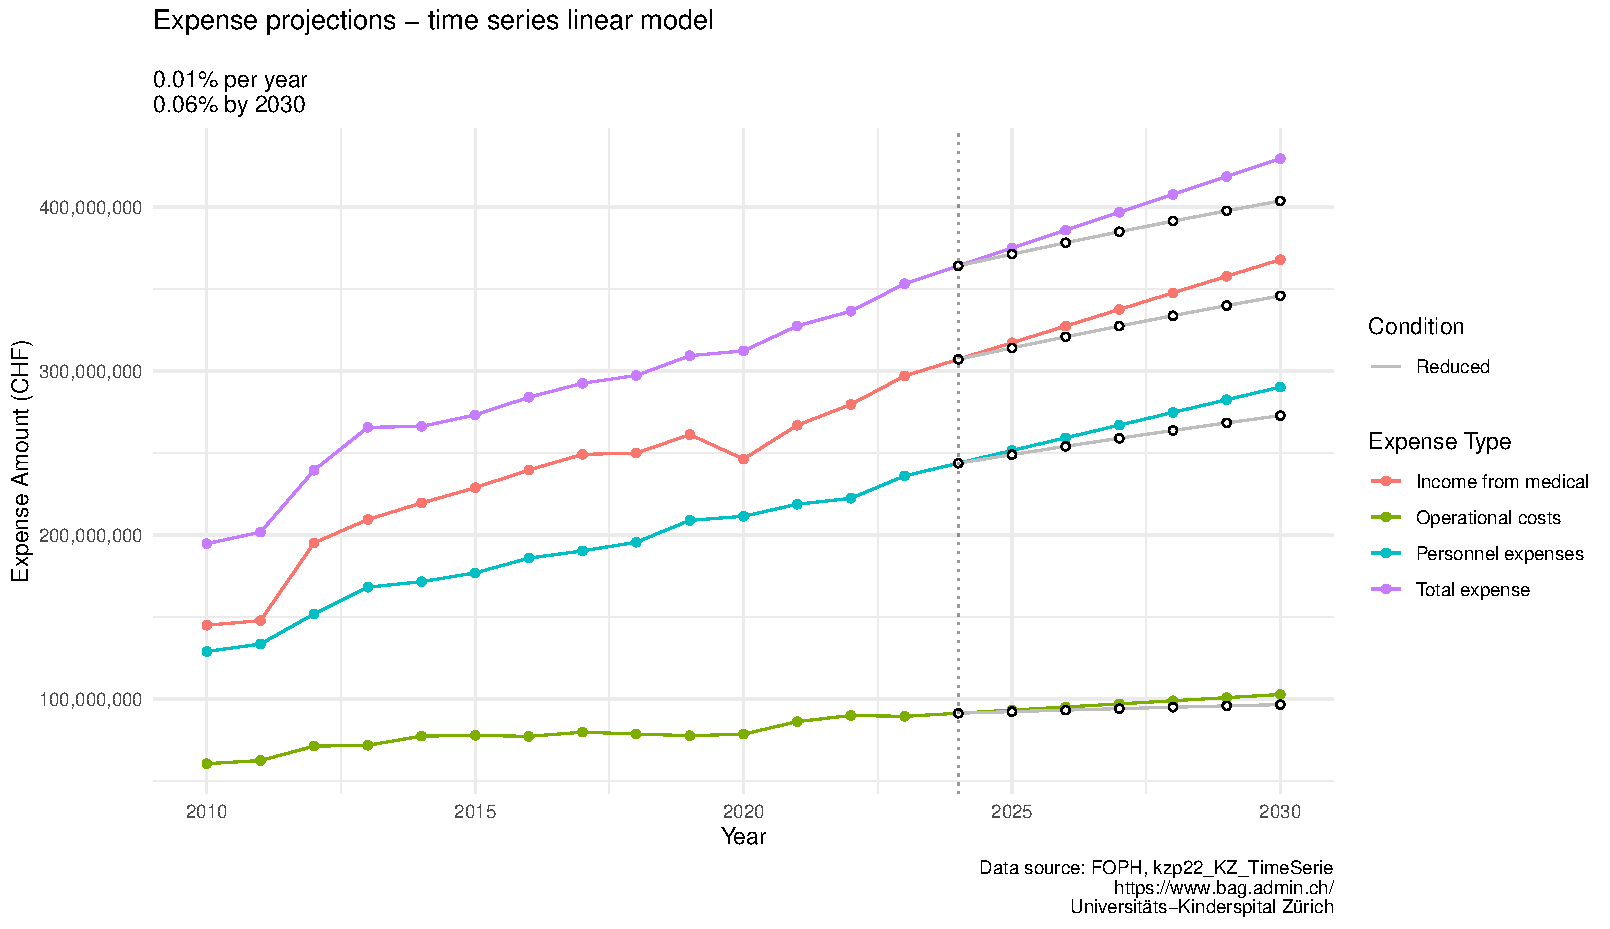
\includegraphics[width=0.90\textwidth]{../../stats/foph_key_stats/output/p_cost}
	\caption{Projections for Kispi with a \pmu (2010-2030). Federal statistics from Bundesamt für Gesundheit (BAG, Federal office for public health) were modelled and projected to 2030. A modest benefit effect size was applied. 
	In the most similar application to our \pmu; 
	\citet{lunke2023integrated} 
	showed a 54\% diagnostic yield and an altered critical care management in 77\% of diagnosed cases.
	We estimated modest 1\% increase in actualised savings per year after successful implementation starting in 2024.}
	\label{fig:cost_analysis}
\end{center}
\end{figure}

A more accurate demonstration of the \pmu can be seen with a specific disease example using sepsis.
Sepsis was specifically modelled using federal statistics from Bundesamt für Gesundheit (BAG, Federal office for public health) from 2010-2022 as shown in 
\textbf{figure
% \ref{fig:p_cases_sepsis_uni_yearly},
\ref{fig:p_cases_sepsis_kispi_yearly_forecast}}.
%\ref{fig:p_cases_per_indicator_kispi_2022}}.
% First we get a global picture of sepsis in University hospitals in  \textbf{figure \ref{fig:p_cases_sepsis_uni_yearly}}.  This illustrates the total number of sepsis in adult and paediatric settings across the country.
The forecast model, from 2010-2030, shows the number of deaths due to sepsis in \kispi (\textbf{Figure \ref{fig:p_cases_sepsis_kispi_yearly_forecast}}).
The predicted number of preventable deaths is based on comparable benchmarks listed in section 
\textbf{\ref{sec:benchmarks}}
which have demonstrated clear cost-saving potential through precise diagnostics and targeted therapy.
For rare diseases, approximately 40\% of probands received a genetic diagnosis 
\citep{wright2023genomic, wojcik2024genome}
and altered critical care management in 77\% of diagnosed cases \citep{lunke2023integrated}.
A well-managed work-flow can result in rapid whole-genome sequencing with a turnaround of 37 hours on average
 \citep{abou2023rapid}.
Based on such values, the forecast  projected into 2030 shows the yearly cases of sepsis.
Black and red values show the expected number of deaths with and without  precise diagnostics and targeted therapy, respectively. 

%\begin{figure}[h] \hspace*{0cm} 
%\begin{center}
%	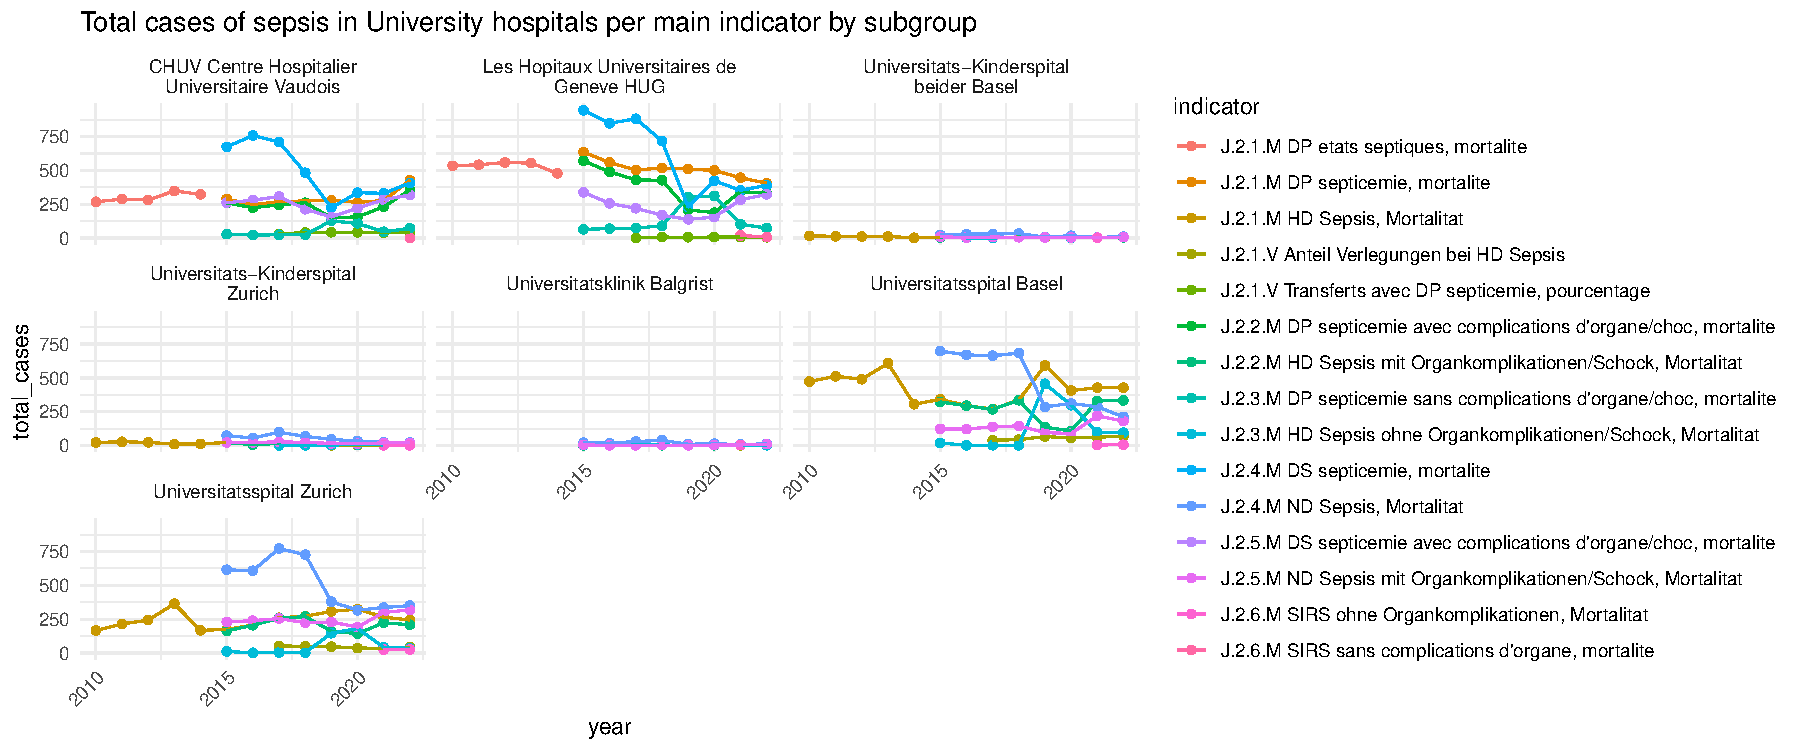
\includegraphics[width=1\textwidth]{../../stats/foph_key_stats/output/p_cases_sepsis_uni_yearly}
%	\caption{Yearly deaths due to sepsis at University hospitals across Switzerland.
%	This data is based on statistics reported by Bundesamt für Gesundheit (BAG), 
%	\url{https://www.bag.admin.ch/} for years 2010-2022. 
%		DP: Diagnostic procedure.
%HD: Primary diagnosis.
%ND: Secondary diagnosis.}
%	\label{fig:p_cases_sepsis_uni_yearly}
%\end{center}
%\end{figure}

\begin{figure}[h] \hspace*{0cm} 
\begin{center}
	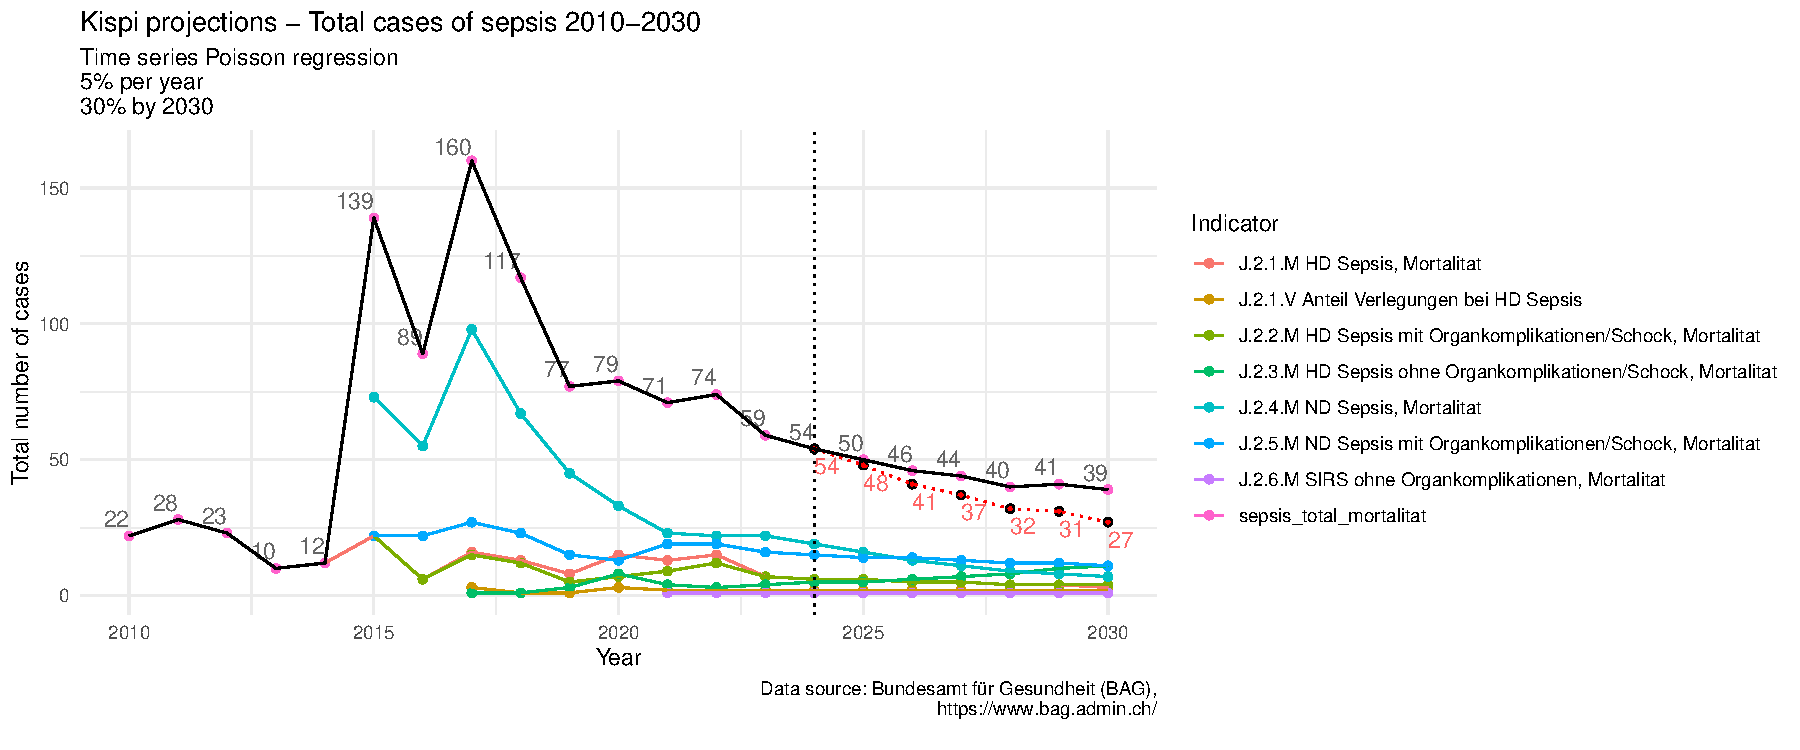
\includegraphics[width=1\textwidth]{../../stats/foph_key_stats/output/p_cases_sepsis_kispi_yearly_forecast}
	\caption{Yearly deaths due to sepsis at \kispi.
	This data is based on statistics reported by Bundesamt für Gesundheit (BAG), 
	\url{https://www.bag.admin.ch/} for years 2010-2022. 
	Time series was performed using Poisson regression to extrapulate the expected outcomes from 2010-2030.
	Predictions for the cost and number of cases were generated in section 
	\ref{sec:benchmarks}.	
	DP: Diagnostic procedure.
HD: Primary diagnosis.
ND: Secondary diagnosis.}
	\label{fig:p_cases_sepsis_kispi_yearly_forecast}
\end{center}
\end{figure}

To put the work of the \pmu in perspective, we look at the total number case statistics for \kispi.
We see a total number of all cases indicators in 2022 of \textbf{10'261}.
The subgroup indicator for ``J.2 sepsis'' shows \textbf{74} cases in 2022.
%\textbf{Figure \ref{fig:p_cases_per_indicator_kispi_2022}}  shows the the indicators through A1-Z4, many of which are similarly affected by the advances in precision medicine and are thus potential future prospects.

%\begin{figure}[h] \hspace*{0cm} 
%\begin{center}
%	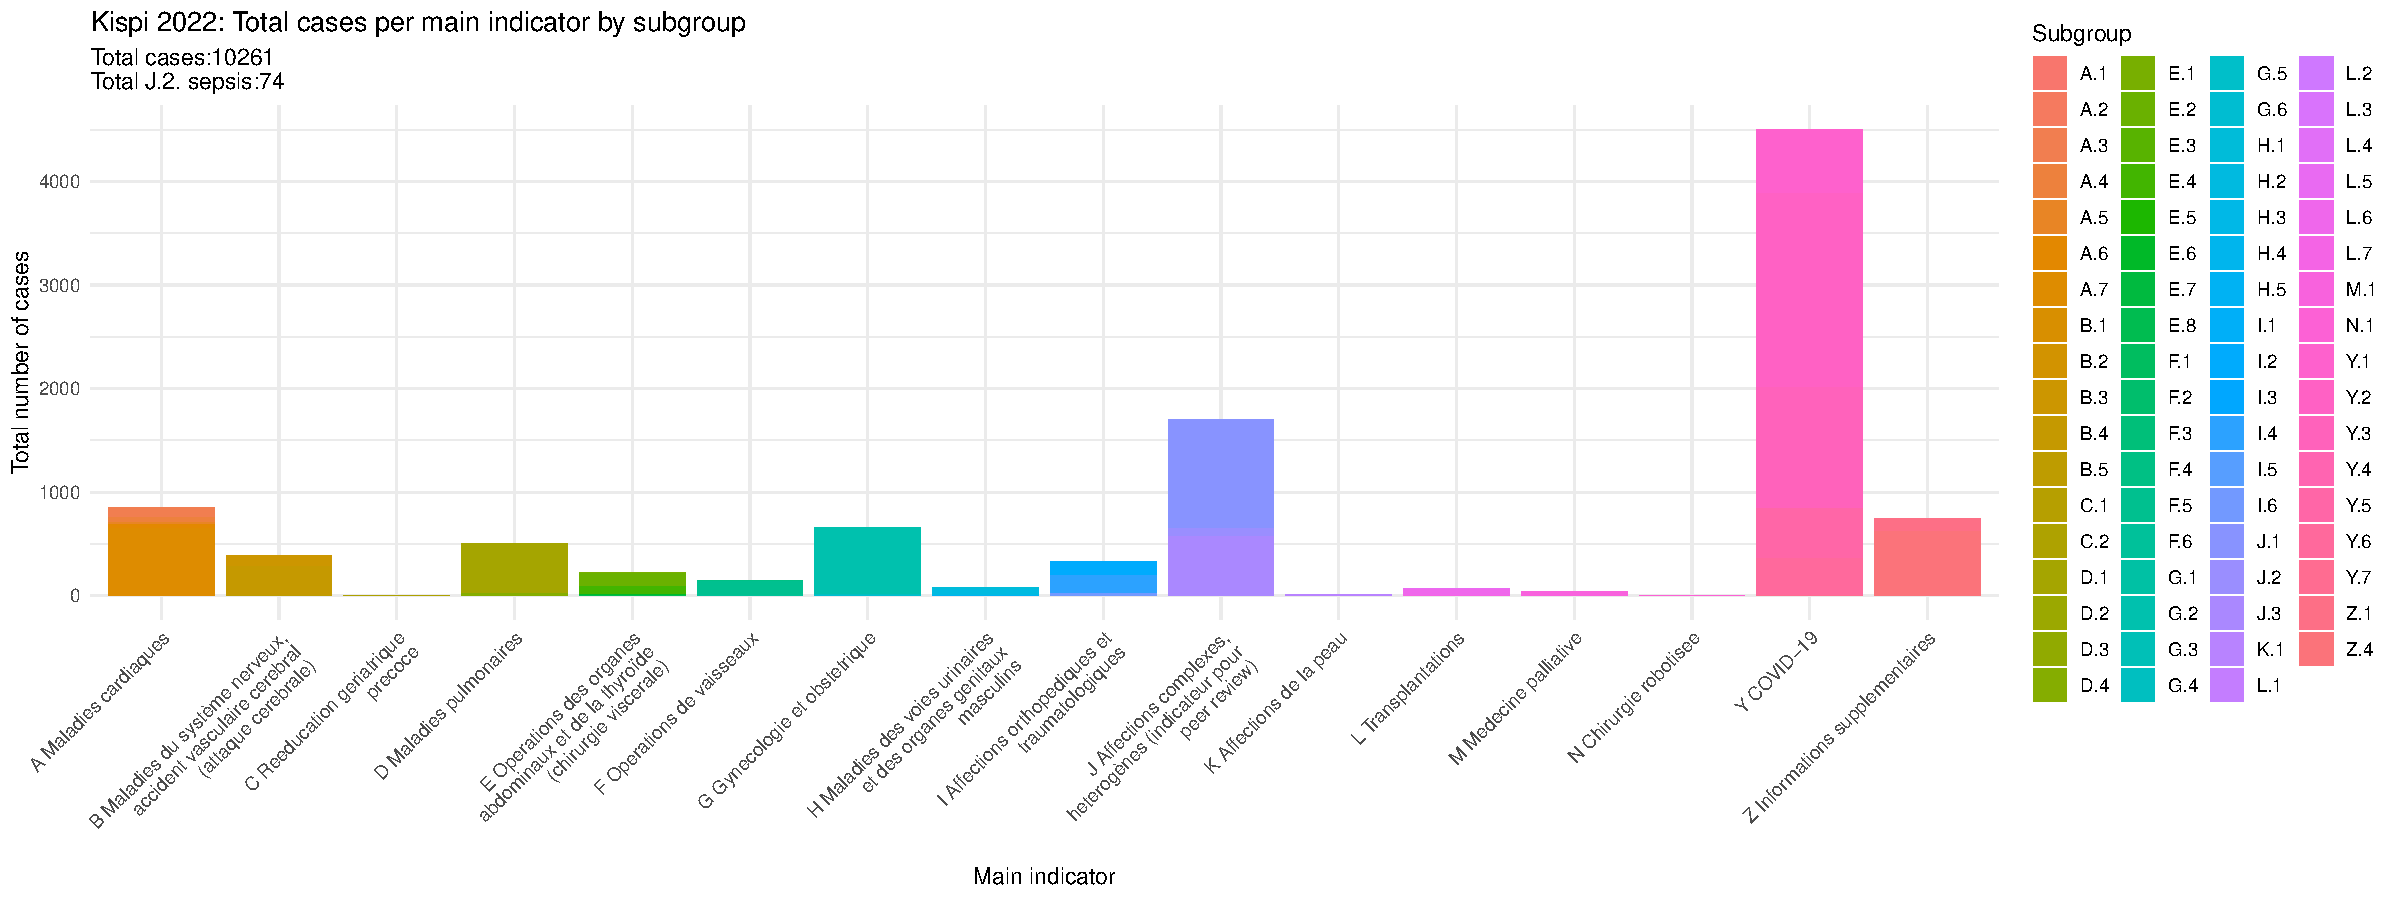
\includegraphics[width=1\textwidth]{../../stats/foph_key_stats/output/p_cases_per_indicator_kispi_2022}
%	\caption{The total count of case descriptions in \kispi for 2022 as categorised according to indicators for the Federal Statistical Office. 
%	The `J.2 Sepsis` subset was used in the other figures shown in this section.}
%	\label{fig:p_cases_per_indicator_kispi_2022}
%\end{center}
%\end{figure}





\section{Collaborations and network}
\subsection{Involved persons}

The GenomeSwift project is supported by a multidisciplinary team of
experts, each bringing unique expertise and experience to ensure the
project\textquotesingle s success. \textbf{Prof. Luregn Schlapbach} will
act as \textbf{mentor}: project management, expected milestones, and
outcomes will be tracked with progress reports. \textbf{Prof. Jacques
Fellay} will provide \textbf{advice} on the tool requirements, essential
guidance on data privacy, consent, and ethical considerations, ensuring
that GenomeSwift adheres to the highest standards of research ethics and
data protection. \textbf{Dr. Dylan Lawless} will act as \textbf{project
leader}: established in genomics and bioinformatics, with extensive
experience in developing computational tools for genomic analysis. He
has expertise in the understanding genetic variations and their
implications in diseases, especially in the context of rare disease in
children. \textbf{Dr. Vito Zanotelli} will act as bioinformatics specialist: he has a
profound understanding of integrating and analysing large-scale genomic
datasets. His expertise is crucial in refining the data processing
algorithms and ensuring that GenomeSwift can handle complex and
voluminous datasets efficiently. 
\textbf{Ali Saadat} has a background in genetic analysis method development, bringing valuable insights into the
clinical implications of genomic findings. His focus is on translating genomic data into actionable clinical knowledge, which is instrumental in designing the interpretative aspects of GenomeSwift. 
\textbf{Dr Zhi Ming Xu} will advise as genomic analysis statistics and software development. A \textbf{PhD student} will be employed to work on development of novel
research features.

Additional collaborating bioinformatics specialists from UZH, ETHZ,
EPFL, and CHUV will integrate and optimise the computational tools
within GenomeSwift. They will test the flow of data in the format
matching our data providers (1) (e.g.,
\href{http://smoc.ethz.ch/}{SwissMultiOmic Center}) to (2) HPC clusters
(e.g., BioMedIT) into (3) GenomeSwift. They will test the clinical
applicability and relevance of the pipeline. Open-source development
will be tested by our collaborators in
\href{https://www.swisspedhealth.ch/}{swisspedhealth.ch}, and
\href{https://www.epfl.ch/labs/fellay-lab/}{EPFL}. Software will be
tested on multiple nodes including ETHZ
\href{https://unlimited.ethz.ch/display/LeoMed2/Leonhard+Med+Intro+for+shareholders}{SIS
Leonhard Med} and University of Basel
\href{https://scicore.unibas.ch/}{sciCORE Med}.


\subsection{National / international collaborations}

GenomeSwift is enhanced by an extensive network of collaborations both
nationally and internationally, significantly impacting healthcare and
research communities. These partnerships facilitate knowledge sharing
and resource exchange, crucial for the project\textquotesingle s
success. \textbf{SwissMultiOmic Center:} Serving as our primary data
provider, this key national partner offers access to state-of-the-art
technologies and datasets, enabling GenomeSwift to utilise high-quality
genomic data and analytical resources. Regular communication between our
groups aids in refining and advancing the pipeline. \textbf{Centre
Hospitalier Universitaire Vaudois (CHUV):} Collaboration with CHUV
researchers to review GenomeSwift\textquotesingle s adaptability across
different healthcare settings, ensuring its effectiveness and
versatility. CHUV's commitment to medical genetics research provides a
solid basis for collaborative enhancements of the pipeline.
\textbf{Ecole Polytechnique Fédérale de Lausanne (EPFL) and ETH Zurich:}
These partnerships grant GenomeSwift access to extensive expertise in
bioinformatics, computational biology, and genomics, fostering a
multidisciplinary integration of varied user needs and methodologies.
\textbf{Global Alliance for Genomics and Health (GA4GH):} GenomeSwift
aligns with GA4GH standards to enhance data interoperability and
security worldwide (\url{https://www.ga4gh.org}). This partnership
ensures GenomeSwift\textquotesingle s integration into global genomic
databases, adhering to international best practices in data privacy and
ethics, thereby contributing to the global \textquotesingle internet of
genomics\textquotesingle. \textbf{Open-source software community:} As a
collaborative open-source project, GenomeSwift benefits from the
collective insights of a diverse group of developers and researchers,
promoting continuous innovation and ensuring the
platform\textquotesingle s ongoing availability and improvement.

\section{Timeline and milestones}\label{timetable-analysis}

Our project timetable was designed and assessed using the critical path
method (CPM) and program evaluation and review technique (PERT). In
\textbf{Figure 2} (A) we present the network of project activities,
highlighting critical paths crucial for project completion.
\textbf{Figure 2} (B) illustrates the Gantt chart, detailing activity
timelines and critical paths, which we tested for effective project
scheduling. Lastly, \textbf{Figure 2} (C) shows the probabilistic
distribution of project completion time, where we tested the risk and
probability of meeting deadlines. Our analysis using CPM and PERT,
provides the optimal plan to assist in timely delivery of outcomes. With
a calculated probability of completion within 53 weeks at 0.97, the
project is highly likely to finish on time according to the PERT
analysis \citep{ref25}, \citep{ref26}, \citep{ref27}, \citep{ref28}, \citep{ref29}

Figure . Timetable with PERT network and Gantt chart. (A) Network
diagram depicting project activities and critical paths. Critical paths
with time dependencies highlighted by color. (B) Gantt chart
illustrating project timelines and critical paths. (C) Probability
distribution of project completion time for risk assessment and deadline
management. CR, time-critical; NC, non-critical.

\section{Financial plan and budget}\label{budget}

\hypertarget{available-resources}{%
\subsection{Available resources}\label{available-resources}}

The GenomeSwift project will use existing resources and infrastructure
available through our collaborations and institutional support, ensuring
a cost-effective approach to its development and implementation.
\textbf{Institutional support}: Access to computational resources and
infrastructure provided by our collaborating institutions, including the
\href{http://smoc.ethz.ch/}{SwissMultiOmic Center}, ETHZ
\href{https://unlimited.ethz.ch/display/LeoMed2/Leonhard+Med+Intro+for+shareholders}{SIS
Leonhard Med}, and University of Basel
\href{https://scicore.unibas.ch/}{sciCORE Med}. \textbf{Existing
grants}: We will also performed development as part of current funding
from related projects within our group which can be found at their
respective research project pages:
\href{https://www.swisspedhealth.ch/}{swisspedhealth.ch}, and
\href{https://www.epfl.ch/labs/fellay-lab/}{EPFL},
\href{https://www.chuv.ch/en/bdsc/research/our-groups/precision-medicine}{CHUV}.

\hypertarget{requested-resources}{%
\subsection{Requested resources}\label{requested-resources}}

\hypertarget{personal-costs-including-social-security-contributions}{%
\subsubsection{Personal costs (including social security
contributions)}\label{personal-costs-including-social-security-contributions}}

A senior staff scientist and a PhD student will each be employed 50\%
FTE to work on development, including social security contributions.
Additional funding is not required for the following: the main applicant
who will oversee the project, collaborating bioinformatics specialists
from UZH, ETHZ, EPFL, and CHUV who will integrate and optimise the
computational tools within GenomeSwift under their current roles within
their respective institutions; our collaborating clinical geneticists
who will review the clinical applicability and relevance of the
pipeline. Total personal costs are 90'448 CHF.

\hypertarget{material-costs}{%
\subsubsection{Material costs}\label{material-costs}}

Costs associated with high-performance computing (HPC) resources for
data processing and analysis are listed in Table 1, including discounts
covered by institutional support. Total costs are 7'628.

\hypertarget{summary-budget-table}{%
\subsection{Summary budget table}\label{summary-budget-table}}

\begin{longtable}[]{@{}
  >{\raggedright\arraybackslash}p{(\columnwidth - 2\tabcolsep) * \real{0.7896}}
  >{\raggedright\arraybackslash}p{(\columnwidth - 2\tabcolsep) * \real{0.2104}}@{}}
\toprule()
\begin{minipage}[b]{\linewidth}\raggedright
1 year project costs
\end{minipage} & \begin{minipage}[b]{\linewidth}\raggedright
~
\end{minipage} \\
\midrule()
\endhead
Senior staff (107\textquotesingle729) 50\% FTE & 53865 \\
Social security contributions (estimated 16\%) & 8618 \\
Postdocs (i.e. 91\textquotesingle280) & 0 \\
Salary for doctoral student (i.e. 48\textquotesingle216) 50\% FTE &
24108 \\
Social security contributions (estimated 16\%) & 3857 \\
Other & ~ \\
Total Direct Costs for Personnel & 90448 \\
Material costs & ~ \\
HPC GPU time & 1520 \\
HPC compute time & 2008 \\
HPC storage 30 TB & 2100 \\
HPC configuration and support & 1000 \\
HPC access services & 1000 \\
Total material costs & 7628 \\
Total & 98076 \\
\bottomrule()
\end{longtable}

\section{References}
 \bibliographystyle{unsrtnat}
\bibliography{references}

\end{document}
